\documentclass[xcolor=x11names,compress]{beamer}
 
%% General document %%%%%%%%%%%%%%%%%%%%%%%%%%%%%%%%%%
\usepackage[utf8]{inputenc}
\usepackage[english,ngerman]{babel}
\usepackage{graphicx}
\usepackage{color}
\usepackage{tikz}
\usepackage{graphicx}
\usepackage{url}

%%%%%%%%%%%%%%%%%%%%%%%%%%%%%%%%%%%%%%%%%%%%%%%%%%%%%%


%% Beamer Layout %%%%%%%%%%%%%%%%%%%%%%%%%%%%%%%%%%
\useoutertheme[subsection=false,infolines]{miniframes}
\useinnertheme{default}
\usefonttheme{serif}
\usepackage{palatino}

\setbeamertemplate{footline}[frame number]
\setbeamertemplate{caption}[numbered]

\setbeamerfont{title like}{shape=\scshape}
\setbeamerfont{frametitle}{shape=\scshape}

\setbeamercolor*{lower separation line head}{bg=DeepSkyBlue4} 
\setbeamercolor*{normal text}{fg=black,bg=white} 
\setbeamercolor*{alerted text}{fg=red} 
\setbeamercolor*{example text}{fg=black} 
\setbeamercolor*{structure}{fg=black} 
 
\setbeamercolor*{palette tertiary}{fg=black,bg=black!10} 
\setbeamercolor*{palette quaternary}{fg=black,bg=black!10} 

\renewcommand{\(}{\begin{columns}}
\renewcommand{\)}{\end{columns}}
\newcommand{\<}[1]{\begin{column}{#1}}
\renewcommand{\>}{\end{column}}


\beamertemplatenavigationsymbolsempty
\setcounter{tocdepth}{1}

\setbeamercolor{page number in head/foot}{fg=black}
\definecolor{bordeaux}{rgb}{0.71,0.01,0.29}
\definecolor{codebg}{rgb}{0.82,0.82,0.82}
\definecolor{codehighlight}{HTML}{D4772A}

%%%%%%%%%%%%%%%%%%%%%%%%%%%%%%%%%%%%%%%%%%%%%%%%%%


\begin{document}



\begin{frame}[plain]
  \begin{figure}
    \flushright
      
\includegraphics[scale=0.12]{hu_logo}
    \vspace*{-0.4cm}
  \end{figure}

  \title{\textbf{Bosch's CAN bus\\Investigation of the standard}\\\vspace{0.2cm}}

  \author{Meryem Can\\Stephan Fahrenkrog-Petersen\\Jakob Rüßler\\Thomas Schlegel\\
  Daniel Titz\\Duc Anh Tran\\\vspace{0.3cm}}

\selectlanguage{english}

\date{\today}
\titlepage
\end{frame}

\begin{frame}
\frametitle{Content}
\tableofcontents[]
\end{frame}

\section{\scshape Introduction}
\begin{frame}
  \frametitle{Introduction and Basic Concepts}
  \begin{itemize}
      \item Controller Area Network 
      \item Serial communications protocol/bus system
      \item Supports distributed realtime control with a very high level of security  ~\cite{can}
   
  \end{itemize}

\end{frame}


\begin{frame}
  \frametitle{Purpose and Context }
  \begin{itemize}
      \item Created by BOSCH
      \item Used in the automotive industry, automation engineering, medical technology, aerospace engineering
      \item Connecting automotive electronics, engine control units, sensors, anti-skid-systems
      \item High speed networks to low cost multiplex wiring
  \end{itemize}

\end{frame}

\begin{frame}
  \frametitle{Related standards}
  \begin{itemize}
      \item standardized after ISO 11898
      \item ISO 11898-2 (Highspeed-CAN) - related
      \item ISISO 11898-3 (Lowspeed-CAN)- related      
      \item Not compitable with each other
  \end{itemize}

\end{frame}

\begin{frame}
  \frametitle{higher standards}
  \begin{itemize}
      \item 
      \item 
      \item     
      \item 
  \end{itemize}

\end{frame}

\section{\scshape Documentation}

\section{\scshape Messages}
\begin{frame}
  \frametitle{Message Transfer and Validation -- 1}
  Overview:
  \begin{itemize}
    \item Information is sent in fixed format messages of different but limited lengths
    \item When free, any connected unit may send messages over the bus
    \item The content of the message is named by an identifier
  \end{itemize}

\end{frame}

\begin{frame}
  \frametitle{Message Transfer and Validation -- 2}
  
    \centering
    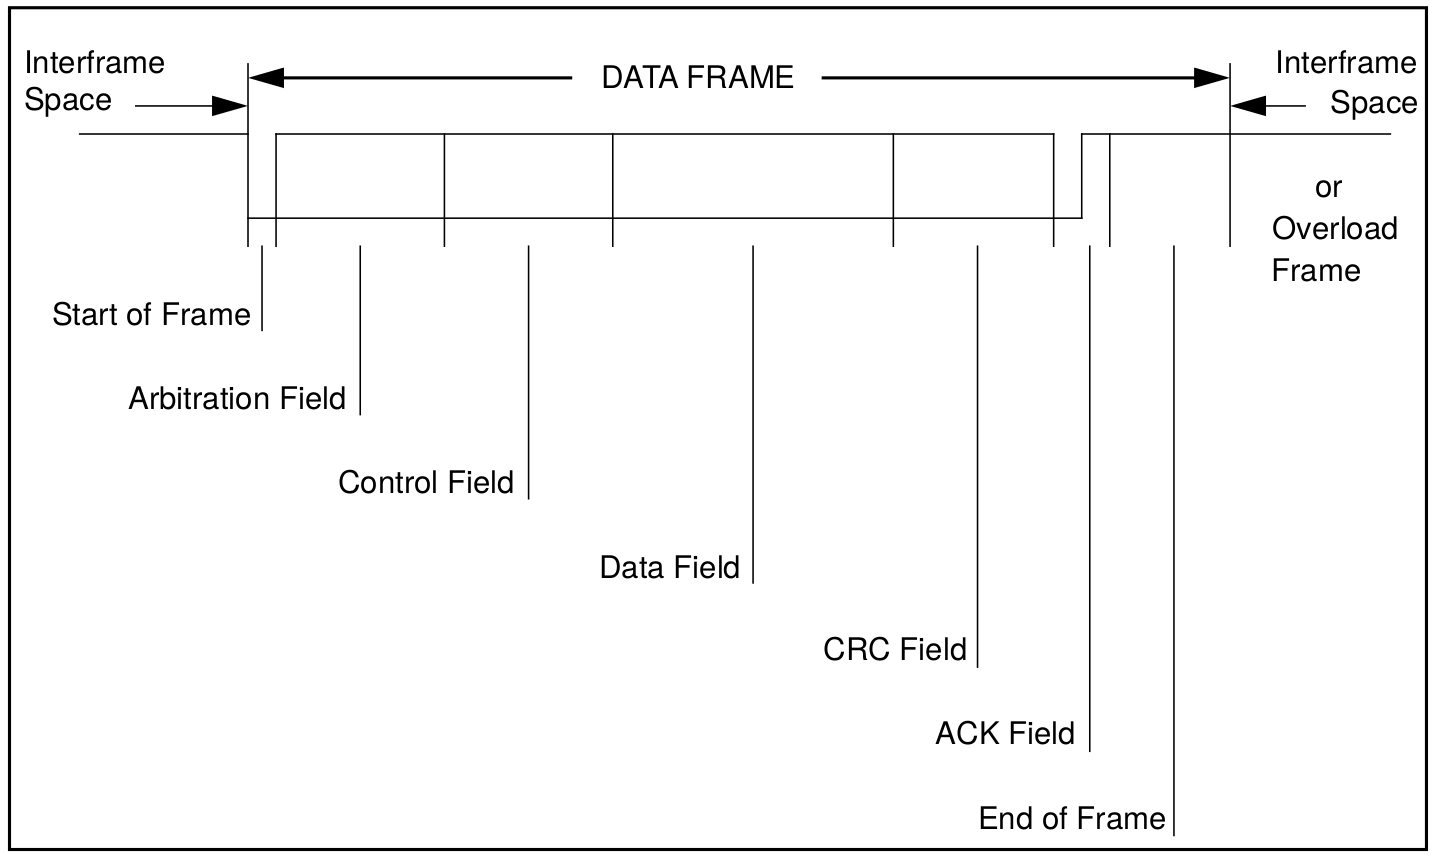
\includegraphics[scale=0.2]{framesetup}

\end{frame}

\begin{frame}
  \frametitle{Message Transfer and Validation -- 3}
  
  \begin{itemize}
    \item A unit sending a message is the ``transmitter'' of that message
    \item It stays transmitter, until the bus is idle or it loses arbitration
    \item A unit is called ``receiver'' of a message, if it is not the transmitter and the bus is not idle
  \end{itemize}

\end{frame}



\section{\scshape Coding / Errors}
\begin{frame}
  \frametitle{Coding and Error Handling -- 1}

  Overview:
  \begin{itemize}
    \item Bit stuffing $\rightarrow$ control mechanism
    \item Distortions etc. $\rightarrow$ error handling to achieve error tolerance
    \item 5 different error types (Bit, Stuff, CRC, Form, ACK)
  \end{itemize}

\end{frame}

\begin{frame}
  \frametitle{Coding and Error Handling -- 2}

  \begin{itemize}
    \item Message passing mechanism, no additional structure needed
    \item Errors broadcasted when detected
    \item Semantics important for correct transmission
    \item Drivers: reliability, error limitation
    \item Problem: new error types?
  \end{itemize}

\end{frame}


\section{\scshape Fault Confinement}
\begin{frame}
  \frametitle{Fault Confinement}
  
    \begin{itemize}
    \item Unit can have 3 states and 2 counters
    \item Strength: Enables extensibility
    \item Drivers: Seperation of concern, reliability, error limitation
    \item Problem: More Unit means more errors?
  \end{itemize}

\end{frame}


\section{\scshape Bit Timing}
\begin{frame}
  \frametitle{Bit Timing Requirements}


\begin{itemize}
    \item List of definitions and rules
    \item Strength: short, but includes everything important
    \item Weaknesses: almost text only, hard to read (structure),
        like a glossary
    \item Improvable by usage of more pictures and examples

\end{itemize}


\end{frame}


\section{\scshape CAN Oscillator}
\begin{frame}
  \frametitle{CAN Improvements}
\end{frame}

\section{\scshape Conclusion}

\begin{frame}
  \frametitle{Conclusion}
\end{frame}

\begin{frame}
  \frametitle{References}
  \scriptsize
  \bibliographystyle{unsrt}
  \bibliography{references}
\end{frame}

\end{document}
